\documentclass[preprint,12pt]{elsarticle}

% Basic packages
\usepackage[a4paper, margin=1in]{geometry}
\usepackage{graphicx}
\graphicspath{{figures/}}
\usepackage{amsmath}
\usepackage{hyperref}
\usepackage{longtable}
\usepackage{booktabs}
\usepackage{caption}
\usepackage{subcaption}
\usepackage{overpic}
\captionsetup[table]{skip=10pt}

% Add Unicode support
\usepackage[utf8]{inputenc}
\usepackage[T1]{fontenc}
\usepackage{textcomp}

% Add color support
\usepackage{xcolor}

% Line numbering
\usepackage{lineno}
\leftlinenumbers
\renewcommand\linenumberfont{\normalfont\small\color{gray}}

% Add support for text formatting
\usepackage{array}
\usepackage{enumitem}
\usepackage{float}

% Add support for special characters
\usepackage{textcomp}
\usepackage{gensymb}


% Citas en texto tipo APA (p.ej., \citep{key} -> (Gonzales et al., 2023))
\biboptions{authoryear,round,semicolon}

%-----------------------------------------------
% METADATA
\title{add title here}

\author[1,2,3]{Javier Lopatin\corref{cor1}}
\ead{javier.lopatin@uai.cl}

%\author[4]{Rocío Araya-López}
%\ead{ro.arayalopez@gmail.com}

%\author[2,5]{Dylan Craven}
%\ead{dylan.craven@umayor.cl}

\address[1]{Faculty of Engineering and Science, Adolfo Ibáñez University, Av. Diagonal Las Torres 2460, Santiago, Chile, 7941169}

\address[2]{Data Observatory Foundation, ANID Technology Center No. DO210001, Santiago, Chile, 7510277}

\address[3]{Center for Climate Resilience Research (CR)2, University of Chile, Santiago, Chile, 8370449}

%\address[4]{Deakin  Marine Research and Innovation Centre, School of Life and Environmental Sciences, Deakin University, Burwood Campus, Burwood, VIC 3125, Australia}

%\address[5]{GEMA Center for Genomics, Ecology and the Environment, Universidad Mayor, Santiago, Chile}

% AGREGAR CORRESPONDING AUTHOR CON COR1
\cortext[cor1]{Corresponding author; javier.lopatin@uai.cl}

%-----------------------------------------------
\begin{document}
\begin{frontmatter}

\begin{abstract}
Hyperspectral reflectance spectroscopy enables non-destructive estimation of plant functional traits, yet current deep learning approaches process spectra as one-dimensional sequences, limiting their capacity to capture long-range inter-band dependencies. We investigated whether transforming 1D hyperspectral signals into 2D image representations improves multi-trait retrieval when coupled with convolutional neural networks. Six transformation methods---direct Reshape, Continuous Wavelet Transform, Multi-Window Spectrogram, Two-Dimensional Correlation Spectroscopy, Gramian Angular Fields, and Markov Transition Field---were systematically compared using EfficientNet-B0 on the GreenHyperSpectra dataset (7,897 labeled spectra, eight traits, 400--2450 nm). \jl{We compared 1D vs 2D CNN models trained from scratch, and models using self-supervised learning using a pretrained masked autoencoder (MAE)}. The simple Reshape transformation achieved the best performance \jl{when tuned from scratch }($R^2 = 0.684 \pm 0.001$), significantly improving all other transforms and the state-of-the-art 1D baseline ($R^2 = 0.587$, $+0.097$). For the self-supervised learning, we tested a pretrained masked autoencoder (MAE-2D) on 139,000 unlabeled spectral images. Linear probing of the frozen encoder ($R^2 = 0.646$) exceeded all MAE-1D methods, including the fine-tuned 1D masked autoencoder ($R^2 = 0.645$), demonstrating that 2D encoders learn high-quality spectral representations \jl{even with the encoder kept frozen and no fine-tuning} \sm{NO ES LO MISMO?}. Our results show that the representational advantage of 2D spectral images, rather than architectural complexity or transfer from natural images, drives the performance gain over 1D approaches.


\end{abstract}

\begin{keyword}
spectral variation hypothesis \sep EnMAP \sep structural equation modeling \sep Mediterranean Andes \sep spatial autocorrelation
\end{keyword}

\end{frontmatter}

\linenumbers

% AGREGAR SECCIONES DE PAPER ACA
\section{Introduction}
\label{sec:introduction}

Plant functional traits are measurable properties that influence how organisms respond to and affect their environment, and are central to understanding ecosystem functioning, biodiversity, and the global carbon cycle \citep{kattge2020try}. \jl{In particular,} traits such as leaf chlorophyll content, carotenoid concentration, leaf mass per area, and leaf area index govern photosynthetic capacity, light interception, and nutrient cycling, making their accurate quantification essential for ecological research and precision agriculture \citep{homolova2013review}. \jl{To meet this need,} hyperspectral reflectance spectroscopy offers a non-destructive pathway for estimating these traits at scale, since foliar biochemistry and canopy structure imprint characteristic absorption features across the 400--2500\,nm spectral range \citep{curran1989imaging, fu2020photosynthetic}. \sm{SUENA MUY CORTADO COMO FRASE TRAS FARASE SIN CONEXION}

Traditional approaches for deriving traits from spectra rely on vegetation indices, look-up table inversion of radiative transfer models such as PROSAIL \citep{feret2021prospectpro, ferreira2025enhancing}, or statistical methods---principally partial least squares regression (PLSR)---that project the high-dimensional spectral space onto a low-dimensional latent representation \citep{fu2020photosynthetic, ji2024unveiling}. While effective, PLSR models are typically trained and validated on individual traits, require careful feature engineering, and can struggle to capture the non-linear relationships between reflectance and biochemical concentrations that arise from multiple scattering and overlapping absorption features \citep{verhoef2007sail}. More recently, one-dimensional convolutional neural networks (1D-CNNs) have been applied directly to spectral vectors, learning hierarchical features end-to-end and achieving state-of-the-art multi-trait retrieval performance without manual feature selection \citep{cherif2023spectra, furbank2021wheat}. \citet{cherif2023spectra} demonstrated that a single EfficientNet-based 1D-CNN trained simultaneously on 20 traits across 50 heterogeneous field datasets outperformed PLSR baselines, establishing a benchmark for transferable multi-trait models. Their subsequent \texttt{GreenHyperSpectra} dataset \citep{cherif2025greenhyperspectra} further advanced this line of work by incorporating semi-supervised and self-supervised pretraining strategies, with a 1D masked autoencoder (MAE) achieving the best results ($R^2 = 0.645$) after fine-tuning on labeled data.

Despite this progress, 1D-CNNs process the spectrum as a flat sequence, inherently limiting their receptive field to local neighbourhoods of adjacent bands. Spectral signatures of plant traits, however, arise from the interplay of multiple absorption features distributed across the full wavelength range---for example, the joint influence of pigment absorption in the visible, water absorption in the shortwave infrared, and structural scattering near the red edge \citep{curran1989imaging, homolova2013review}. Capturing these long-range inter-band dependencies within a 1D framework requires either very deep networks or large kernel sizes, both of which increase the risk of overfitting when labeled training data are scarce.

An alternative strategy, increasingly explored in signal processing and chemometrics, is to transform one-dimensional signals into two-dimensional image representations and leverage the powerful feature extraction capabilities of 2D-CNNs originally developed for computer vision \citep{wang2015gaf, garcia2022temporal}. Several encoding methods have been proposed for this purpose. Gramian Angular Fields (GAF) and Markov Transition Fields (MTF) encode temporal or spectral correlations as square images by mapping signal values to angular or transition-probability spaces \citep{wang2015gaf, ganesan2021gaf}. Continuous wavelet transform (CWT) scalograms decompose signals across multiple frequency scales, producing time-frequency representations that have proven effective for fault diagnosis, medical signal classification, and spectral analysis \citep{addison2017wavelet, Lopatin2023-fn, ong2025sugarcane, zhuang2023cwt}. Short-time Fourier transform spectrograms offer a complementary multi-window decomposition \citep{shuai2025multichannel}, while direct reshaping---simply folding the 1D vector into a 2D matrix---has been shown to produce surprisingly competitive results by preserving wavelength adjacency as spatial texture \citep{hennessy2022reshaping, deev2024spectrum, sharma2019deepinsight}. More recently, these encoding techniques have begun to appear in spectroscopic applications, including GAF-based adulteration detection in food products \citep{zhang2025gaf} and CWT-assisted disease recognition from near-infrared spectra \citep{ong2025sugarcane}.

However, the application of 1D-to-2D spectral transformations to vegetation trait retrieval from hyperspectral data remains largely unexplored. Existing studies in this domain have predominantly focused on classification tasks (e.g., species discrimination) rather than continuous regression of biophysical variables \citep{hennessy2022reshaping}, and no systematic comparison of multiple transformation methods under controlled experimental conditions has been conducted. Furthermore, the conversion of spectra to 2D images unlocks capabilities exclusive to the vision domain that are inaccessible to 1D spectral architectures. \jl{The most important of these is} the ability to leverage self-supervised pretraining with 2D masked autoencoders \citep{he2022mae}, which have demonstrated remarkable success in learning visual representations from unlabeled image data. While 1D MAEs have been applied to spectral pretraining \citep{cherif2025greenhyperspectra}, the potential of 2D MAEs operating on transformed spectral images has not been investigated.

In this study, we aim to: (i) systematically compare the performance of six 1D-to-2D spectral transformation methods as spectral encoding strategies for 2D-CNN-based trait retrieval; and (ii) assess whether converting spectra to 2D images enables self-supervised pretraining via masked autoencoders to improve trait predictions beyond what 1D pretraining achieves. We used the \texttt{GreenHyperSpectra} dataset to benchmark our 2D approach against the state-of-the-art 1D methods \citep{cherif2025greenhyperspectra}. 

\section{Methods}
\label{sec:methods}

\subsection{Study Data}
\label{sec:data}

We used the GreenHyperSpectra dataset \citep{cherif2025greenhyperspectra}, a large-scale multi-source hyperspectral collection recently published as a benchmarking resource for plant trait prediction. The dataset comprises two components: a labeled set of 7,897 vegetation canopy reflectance spectra with co-located measurements of seven functional plant traits, and an unlabeled set of 139,295 spectra collected from proximal, airborne, and spaceborne platforms across diverse continents, ecosystems, and sensor configurations. All spectra were resampled to a uniform wavelength grid spanning 400--2450\,nm at 1\,nm resolution. Regions of strong atmospheric water absorption (1351--1430\,nm, 1801--2050\,nm, and 2451--2500\,nm) were removed, and a Savitzky-Golay smoothing filter (window = 65, polynomial order = 1) was applied per spectral segment, yielding 1721 spectral bands per sample \citep{cherif2025greenhyperspectra}.

The labeled subset aggregates data from 50 field campaigns spanning forests, grasslands, croplands, tundra, and pastures, with trait values harmonized to area-based units. The seven target traits correspond to parameters of the PROSPECT-PRO radiative transfer model \citep{feret2021prospectpro}: leaf chlorophyll content (C\textsubscript{ab}, $\mu$g\,cm\textsuperscript{$-$2}), carotenoid content (C\textsubscript{ar}, $\mu$g\,cm\textsuperscript{$-$2}), anthocyanin content (C\textsubscript{anth}, $\mu$g\,cm\textsuperscript{$-$2}), equivalent water thickness (C\textsubscript{w}, g\,m\textsuperscript{$-$2}), leaf mass per area (C\textsubscript{m}, g\,m\textsuperscript{$-$2}), leaf area index (LAI, m\textsuperscript{2}\,m\textsuperscript{$-$2}), and protein content (C\textsubscript{p}, g\,m\textsuperscript{$-$2}). An eighth derived trait, carbon-based constituents (C\textsubscript{bc} = C\textsubscript{m} $-$ C\textsubscript{p}), was additionally computed following \citet{cherif2025greenhyperspectra}. Not all samples possess measurements for every trait; the dataset is inherently sparse, with missing values handled through masked loss functions during training (Section~\ref{sec:training}).

For model evaluation, we adopted the standardized data split provided with GreenHyperSpectra: a stratified 80/20 partition yielding 4,508 training and 1,127 test samples, with stratification by source dataset to maintain proportional representation of vegetation types, sensors, and acquisition conditions across both subsets. To quantify variability due to stochastic training effects, all experiments were repeated across three random seeds (155, 240, and 318), following the evaluation protocol of \citet{cherif2025greenhyperspectra}.


\subsection{1D-to-2D Spectral Transformations}
\label{sec:transforms}

The central premise of this work is that converting one-dimensional hyperspectral reflectance signals into two-dimensional image representations may reveal inter-band relationships, multi-scale spectral patterns, and structural regularities that conventional 1D convolutional architectures fail to capture. We evaluated six transformation methods, each encoding different aspects of the spectral information into spatial image structure. All transformations produced images of $224 \times 224$ pixels (with varying numbers of channels) suitable for standard convolutional neural network architectures.

\subsubsection{Direct Reshape}

The simplest transformation reshapes the 1D spectral vector into a 2D matrix by computing the smallest integer side length $s = \lceil\sqrt{n}\rceil$ where $n = 1721$ bands, yielding $s = 42$. The spectrum is zero-padded to $42 \times 42 = 1764$ elements (appending 43 zeros) and folded into a square matrix, which is then bilinearly resized to $224 \times 224$ and min-max normalized to $[0, 1]$. Despite its simplicity, this transformation preserves the sequential ordering of wavelengths, such that spatially adjacent pixels correspond to spectrally proximate bands. The resulting single-channel image encodes local spectral gradients as spatial texture that 2D convolutions can exploit.

\subsubsection{Continuous Wavelet Transform}

The continuous wavelet transform (CWT) decomposes the spectral signal across multiple frequency scales simultaneously, producing a time-frequency (or in this case, wavelength-scale) representation known as a scalogram \citep{addison2017wavelet}. We employed the Morlet wavelet across 128 logarithmically spaced scales ranging from 1 to 128, computed using the PyWavelets library \citep{pywt}. The absolute values of the wavelet coefficients form a $128 \times 1721$ scalogram that captures both narrow absorption features (at fine scales) and broad spectral trends (at coarse scales). The scalogram was bilinearly resized to $224 \times 224$ and min-max normalized, yielding a single-channel image.

\subsubsection{Multi-Window Spectrogram}

The short-time Fourier transform (STFT) was applied with three different window functions---Bartlett, Gaussian ($\sigma = 12$), and Blackman---each producing a complementary time-frequency representation of the spectrum. We used a segment length of 64 samples with 50\% overlap (32 samples), following the multi-channel approach of \citet{shuai2025multichannel}. The magnitude of each STFT output was computed, bilinearly resized to $224 \times 224$, and min-max normalized. The three resulting spectrograms were stacked as a three-channel (RGB-like) image, where each channel emphasizes different spectral features owing to the distinct frequency leakage and sidelobe characteristics of the respective windows.

\subsubsection{Two-Dimensional Correlation Spectroscopy}

Two-dimensional correlation spectroscopy (2D-COS) generates synchronous and asynchronous correlation maps from perturbation-induced spectral variations \citep{noda2004twodimensional}. We simulated perturbation by dividing each spectrum into 10 overlapping segments (50\% overlap) and computing the cross-correlation between band intensities across segments. The synchronous correlation matrix $\Phi = \mathbf{X}^T \mathbf{X} / (m-1)$, where $\mathbf{X}$ is the mean-centered segment matrix and $m$ is the number of segments, captures in-phase inter-band correlations. The asynchronous correlation matrix $\Psi = \mathbf{X}^T \mathbf{N} \mathbf{X} / (m-1)$ employs the Hilbert-Noda transformation matrix $N_{ij} = 1/[\pi(j-i)]$ for $i \neq j$ (and zero otherwise), revealing sequential spectral changes. Both matrices were individually min-max normalized and bilinearly resized to $224 \times 224$, then stacked as a two-channel image.

\subsubsection{Gramian Angular Fields}

Gramian Angular Fields (GAF) encode temporal (or spectral) correlations as angular relationships in a polar coordinate system \citep{wang2015gaf}. The spectrum is first downsampled to 224 values via linear interpolation and scaled to $[-1, 1]$. An angular representation $\varphi_i = \arccos(x_i)$ is computed for each spectral value, and two complementary fields are generated: the Gramian Angular Summation Field (GASF), defined as $\text{GASF}_{ij} = \cos(\varphi_i + \varphi_j)$, which captures in-phase spectral correlations; and the Gramian Angular Difference Field (GADF), defined as $\text{GADF}_{ij} = \sin(\varphi_i - \varphi_j)$, which captures phase differences. The two fields were min-max normalized and stacked as a two-channel image.

\subsubsection{Markov Transition Field}

The Markov Transition Field (MTF) encodes the transition dynamics between discretized spectral value bins as a spatial image \citep{wang2015gaf}. The spectrum is downsampled to 224 values and discretized into 8 quantile-based bins. A first-order Markov transition matrix $\mathbf{P}$ is estimated, where $P_{ij}$ represents the conditional probability of transitioning from bin $i$ to bin $j$ across consecutive spectral positions. The MTF is then constructed as $\text{MTF}_{ij} = P[q_i, q_j]$, where $q_i$ and $q_j$ are the bin assignments at spectral positions $i$ and $j$, respectively. The resulting $224 \times 224$ single-channel image was min-max normalized.


\subsection{Model Architectures}
\label{sec:models}

\subsubsection{Supervised Regression: EfficientNet-B0}
\label{sec:efficientnet}

For supervised multi-trait regression, we employed EfficientNet-B0 \citep{tan2019efficientnet} as the backbone architecture, instantiated through the timm library \citep{rw2019timm}. EfficientNet-B0 was selected for its favorable trade-off between model capacity ($\sim$4\,M trainable parameters) and computational efficiency, which proved critical given the moderate size of the labeled training set ($n = 4{,}508$). The network's final classification layer was replaced with a linear head mapping to 8 output neurons (one per target trait), and a dropout rate of 0.3 was applied before the output layer. For single-channel transformations (Reshape, CWT, MTF), the first convolutional layer was adapted from three to one input channel using timm's automatic weight adaptation, which sums the pretrained RGB channel weights along the input dimension. Multi-channel transformations (Spectrogram: 3 channels; 2D-COS and GAF: 2 channels) required analogous channel-count adjustments.

\subsubsection{Self-Supervised Pretraining: Masked Autoencoder (MAE-2D)}
\label{sec:mae}

To leverage the 139,295 unlabeled spectra for representation learning, we implemented a two-dimensional Masked Autoencoder (MAE) following the framework of \citet{he2022mae}. The MAE operates on 2D spectral images produced by the best-performing transformation (Reshape; see Section~\ref{sec:results_transforms}), enabling the use of standard vision transformer components that are unavailable for 1D spectral inputs.

The encoder follows a Vision Transformer (ViT) architecture \citep{dosovitskiy2021vit} with patch size $16 \times 16$, embedding dimension 192, 6 transformer blocks, and 3 attention heads per block, yielding 196 patches per $224 \times 224$ image. During pretraining, 75\% of patches are randomly masked, and only the visible 25\% are processed by the encoder, substantially reducing computational cost. Fixed sinusoidal 2D positional embeddings are added to all patch tokens, and a learnable class (CLS) token is prepended to the sequence.

The decoder is a lightweight transformer with embedding dimension 96, 4 blocks, and 3 attention heads. It receives the encoded visible patches along with learnable mask tokens that replace the masked positions. After processing through the decoder blocks, a linear projection maps each token to the pixel values of its corresponding $16 \times 16$ patch. The reconstruction loss is computed only on masked patches:
\begin{equation}
    \mathcal{L}_\text{MAE} = \frac{1}{|\mathcal{M}|} \sum_{i \in \mathcal{M}} \| \hat{\mathbf{p}}_i - \mathbf{p}_i \|^2
\end{equation}
where $\mathcal{M}$ denotes the set of masked patch indices, $\hat{\mathbf{p}}_i$ is the reconstructed patch, and $\mathbf{p}_i$ is the original patch. No data augmentation beyond random masking was applied during pretraining, consistent with the finding of \citet{he2022mae} that masking itself provides sufficient regularization, and following the protocol of \citet{cherif2025greenhyperspectra} whose 1D MAE likewise omitted augmentation.

The total model comprises approximately 3.3\,M parameters (2.8\,M encoder, 0.5\,M decoder). After pretraining, the decoder is discarded, and the encoder's CLS token representation serves as a global feature vector for downstream trait regression through an appended two-layer MLP head (192 $\rightarrow$ 192 $\rightarrow$ 8, with GELU activation and 10\% dropout).



\subsection{Training Protocol}
\label{sec:training}

All models were implemented in PyTorch 2.6 \citep{paszke2019pytorch} using PyTorch Lightning 2.6 for training orchestration. Pre-computed 2D transformations were stored as memory-mapped arrays to avoid recomputation during training.

\subsubsection{Supervised Training}

The supervised EfficientNet-B0 models were optimized with AdamW \citep{loshchilov2019adamw} ($\beta_1 = 0.9$, $\beta_2 = 0.999$, weight decay = $10^{-4}$) and a cosine annealing learning rate schedule with initial rate $10^{-3}$ and minimum rate $10^{-6}$. Training proceeded for a maximum of 100 epochs with early stopping (patience = 15 epochs, monitoring validation loss). Within the training set, 15\% of samples were withheld for validation using stratified random splitting. The batch size was set to 16 to accommodate GPU memory constraints (NVIDIA RTX 2060, 6\,GB).

Because the trait label matrix is sparse---not all samples have measurements for all eight traits---we employed a masked mean squared error (MSE) loss that computes gradients only over observed trait values:
\begin{equation}
    \mathcal{L}_\text{masked} = \frac{\sum_{i,j} m_{ij}(\hat{y}_{ij} - y_{ij})^2}{\sum_{i,j} m_{ij}}
\end{equation}
where $\hat{y}_{ij}$ and $y_{ij}$ are the predicted and observed values for sample $i$ and trait $j$, and $m_{ij}$ is a binary mask indicating whether the observation is available. Prior to training, trait values were transformed using the Yeo-Johnson power transformation \citep{yeo2000power} fitted on the training set, which stabilizes variance and reduces the influence of skewed distributions. Predictions were inverse-transformed for evaluation in original units.

\subsubsection{MAE Pretraining}

The MAE-2D was pretrained on Reshape images derived from the 139,295 unlabeled spectra (after filtering 375 samples with missing data, yielding 138,920 valid images). Training used AdamW ($lr = 10^{-4}$, weight decay = $10^{-4}$) with cosine annealing over 300 epochs, a batch size of 32, and gradient clipping (max norm = 1.0). A 95/5 train/validation split was used for monitoring reconstruction loss, with early stopping at patience = 30 epochs. The pretraining objective was pure MSE reconstruction of masked patches (Equation~1), without additional augmentation, as random masking already provides effective regularization \citep{he2022mae}.

\subsubsection{Fine-Tuning}

After MAE pretraining, the decoder was discarded and the encoder was equipped with a regression MLP head. Two fine-tuning strategies were evaluated: (i) \textit{full fine-tuning}, where all encoder parameters are updated jointly with the regression head ($lr = 10^{-4}$); and (ii) \textit{linear probing}, where encoder weights are frozen and only the regression head is trained ($lr = 10^{-3}$). Fine-tuning used the same protocol as supervised training (AdamW, early stopping, masked MSE loss) with 100 maximum epochs.


\subsection{Experimental Design}
\label{sec:experimental_design}

The experiments are organized into two complementary case studies that progressively demonstrate the advantages of 2D spectral representations.

\textit{Case Study 1: Transform comparison.} All six 1D-to-2D transformations (Section~\ref{sec:transforms}) were evaluated using EfficientNet-B0 under identical supervised training conditions. The primary comparison is between our 2D approach and the supervised EfficientNet-1D baseline reported by \citet{cherif2025greenhyperspectra} (mean $R^2 = 0.587$ across eight traits). The Reshape transformation, which exhibited the highest mean $R^2$ and lowest variance across seeds, was selected as the representative 2D method for Case Study 2.

\textit{Case Study 2: Self-supervised pretraining.} Two experiments assessed the impact of pretraining strategies, both using Reshape as the fixed transformation: (i) supervised training without pretraining (the Case Study 1 baseline); and (ii) MAE-2D pretraining on 139K unlabeled images followed by fine-tuning on real labeled data, compared against the MAE-1D of \citet{cherif2025greenhyperspectra} ($R^2 = 0.645$).


\subsection{Evaluation Metrics}
\label{sec:metrics}

Model performance was evaluated using the coefficient of determination ($R^2$) and the normalized root mean square error (nRMSE, expressed as percentage of the 1st--99th percentile range of observed values), computed per trait on the held-out test set. We report the mean and standard deviation across three random seeds for all experiments. Per-trait $R^2$ values were averaged to obtain a single summary statistic for each method, enabling direct comparison with the baselines of \citet{cherif2025greenhyperspectra} who used the same evaluation protocol. Additional metrics---root mean square error (RMSE), mean absolute error (MAE), and bias---are reported in supplementary materials for completeness.

\section{Results}
\label{sec:results}

\subsection{Case Study 1: Transform Comparison}
\label{sec:results_transforms}

Table~\ref{tab:transforms} summarizes the performance of all six 1D-to-2D spectral transformations evaluated with EfficientNet-B0 on the GreenHyperSpectra dataset. The direct Reshape transformation achieved the highest mean $R^2$ of 0.684 $\pm$ 0.001 across eight plant traits, representing a substantial improvement of +0.097 over the supervised EfficientNet-1D baseline reported by \citet{cherif2025greenhyperspectra} ($R^2 = 0.587$). Reshape also exhibited the lowest variance across random seeds, indicating robust and reproducible performance. The continuous wavelet transform (CWT, $R^2 = 0.641 \pm 0.004$) and multi-window spectrogram ($R^2 = 0.636 \pm 0.025$) ranked second and third, respectively, though with notably higher inter-seed variability in the case of the spectrogram. The two-dimensional correlation spectroscopy (2D-COS, $R^2 = 0.625$) and Gramian Angular Fields (GAF, $R^2 = 0.623$) yielded moderate improvements over the 1D baseline, while the Markov Transition Field (MTF, $R^2 = 0.426$) was the only transformation that performed substantially worse than the 1D approach.

Five of six transformations surpassed the 1D-CNN baseline, demonstrating that the conversion of hyperspectral signals to two-dimensional image representations captures spectral information that one-dimensional convolutional architectures fail to exploit. The consistent superiority of the simpler Reshape transformation over more computationally intensive methods such as CWT and 2D-COS suggests that preserving the sequential ordering of wavelengths---where spatially adjacent pixels correspond to spectrally proximate bands---provides sufficient spatial structure for 2D convolutions to learn inter-band relationships.

\begin{table}[htbp]
\centering
\caption{Comparison of 1D-to-2D spectral transformations for multi-trait retrieval using EfficientNet-B0 on the GreenHyperSpectra dataset. Mean $R^2$ and standard deviation are reported across three random seeds (155, 240, 318). All methods are compared against the supervised EfficientNet-1D baseline of \citet{cherif2025greenhyperspectra} ($R^2 = 0.587$). The best result per column is shown in bold.}
\label{tab:transforms}
\begin{tabular}{llccr}
\toprule
Transform & Channels & Mean $R^2$ $\pm$ std & $\Delta$ vs.\ 1D & Seeds \\
\midrule
\textbf{Reshape}     & 1 & \textbf{0.684 $\pm$ 0.001} & \textbf{+0.097} & 3 \\
CWT                   & 1 & 0.641 $\pm$ 0.004          & +0.054          & 3 \\
Spectrogram           & 3 & 0.636 $\pm$ 0.025          & +0.049          & 3 \\
2D-COS                & 2 & 0.625                      & +0.038          & 1 \\
GAF                   & 2 & 0.623                      & +0.036          & 1 \\
MTF                   & 1 & 0.426                      & $-$0.161        & 1 \\
\midrule
Cherif 1D-CNN         & -- & 0.587                     & --              & 3 \\
\bottomrule
\end{tabular}
\end{table}


\subsection{Per-Trait Analysis}
\label{sec:results_per_trait}

Table~\ref{tab:per_trait} presents the per-trait comparison between the best 2D method (Reshape) and the 1D baseline. The 2D approach improved retrieval accuracy for all eight traits, with improvements ranging from +0.008 for protein content (C\textsubscript{p}) to +0.245 for carbon-based constituents (C\textsubscript{bc}). The largest gains were observed for traits related to leaf structural composition: C\textsubscript{bc} ($\Delta R^2 = +0.245$), anthocyanins ($\Delta R^2 = +0.174$), and leaf mass per area ($\Delta R^2 = +0.122$). These traits are characterised by broad, overlapping absorption features across multiple spectral regions, suggesting that the 2D representation enables the model to capture cross-band correlations that are informative for their retrieval. Pigment-related traits (chlorophyll, carotenoids) showed moderate improvements (+0.070 to +0.080), while canopy-level traits (LAI, +0.041; equivalent water thickness, +0.036) and protein content (+0.008) exhibited smaller but consistent gains.

\begin{table}[htbp]
\centering
\caption{Per-trait $R^2$ comparison between the best 2D method (Reshape + EfficientNet-B0) and the supervised 1D baseline \citep{cherif2025greenhyperspectra}. Values for the 2D method are averaged across three random seeds; values for Cherif are from their reported results. The best value per trait is shown in bold.}
\label{tab:per_trait}
\begin{tabular}{lccr}
\toprule
Trait & Cherif 1D & Reshape 2D & $\Delta$ \\
\midrule
C\textsubscript{ab} (Chlorophyll)    & 0.517 & \textbf{0.597} & +0.080 \\
C\textsubscript{ar} (Carotenoids)    & 0.621 & \textbf{0.691} & +0.070 \\
C\textsubscript{anth} (Anthocyanins) & 0.454 & \textbf{0.628} & +0.174 \\
C\textsubscript{w} (EWT)             & 0.667 & \textbf{0.703} & +0.036 \\
C\textsubscript{m} (LMA)             & 0.651 & \textbf{0.773} & +0.122 \\
LAI                                   & 0.563 & \textbf{0.604} & +0.041 \\
C\textsubscript{p} (Protein)         & 0.679 & \textbf{0.687} & +0.008 \\
C\textsubscript{bc} (CBC)            & 0.544 & \textbf{0.789} & +0.245 \\
\midrule
\textbf{Mean}                         & 0.587 & \textbf{0.684} & \textbf{+0.097} \\
\bottomrule
\end{tabular}
\end{table}


Figure~\ref{fig:scatterplot} shows observed versus predicted values for all eight traits using the best model configuration (Reshape + EfficientNet-B0). Strong agreement along the 1:1 line is evident for leaf mass per area ($R^2 = 0.773$), carbon-based constituents ($R^2 = 0.787$), and carotenoids ($R^2 = 0.707$). Chlorophyll content ($R^2 = 0.570$) and leaf area index ($R^2 = 0.592$) show greater scatter, particularly at higher observed values, reflecting the inherent difficulty of these retrievals from canopy-level reflectance where saturation effects are well documented \citep{cherif2025greenhyperspectra}.

\begin{figure}[htbp]
    \centering
    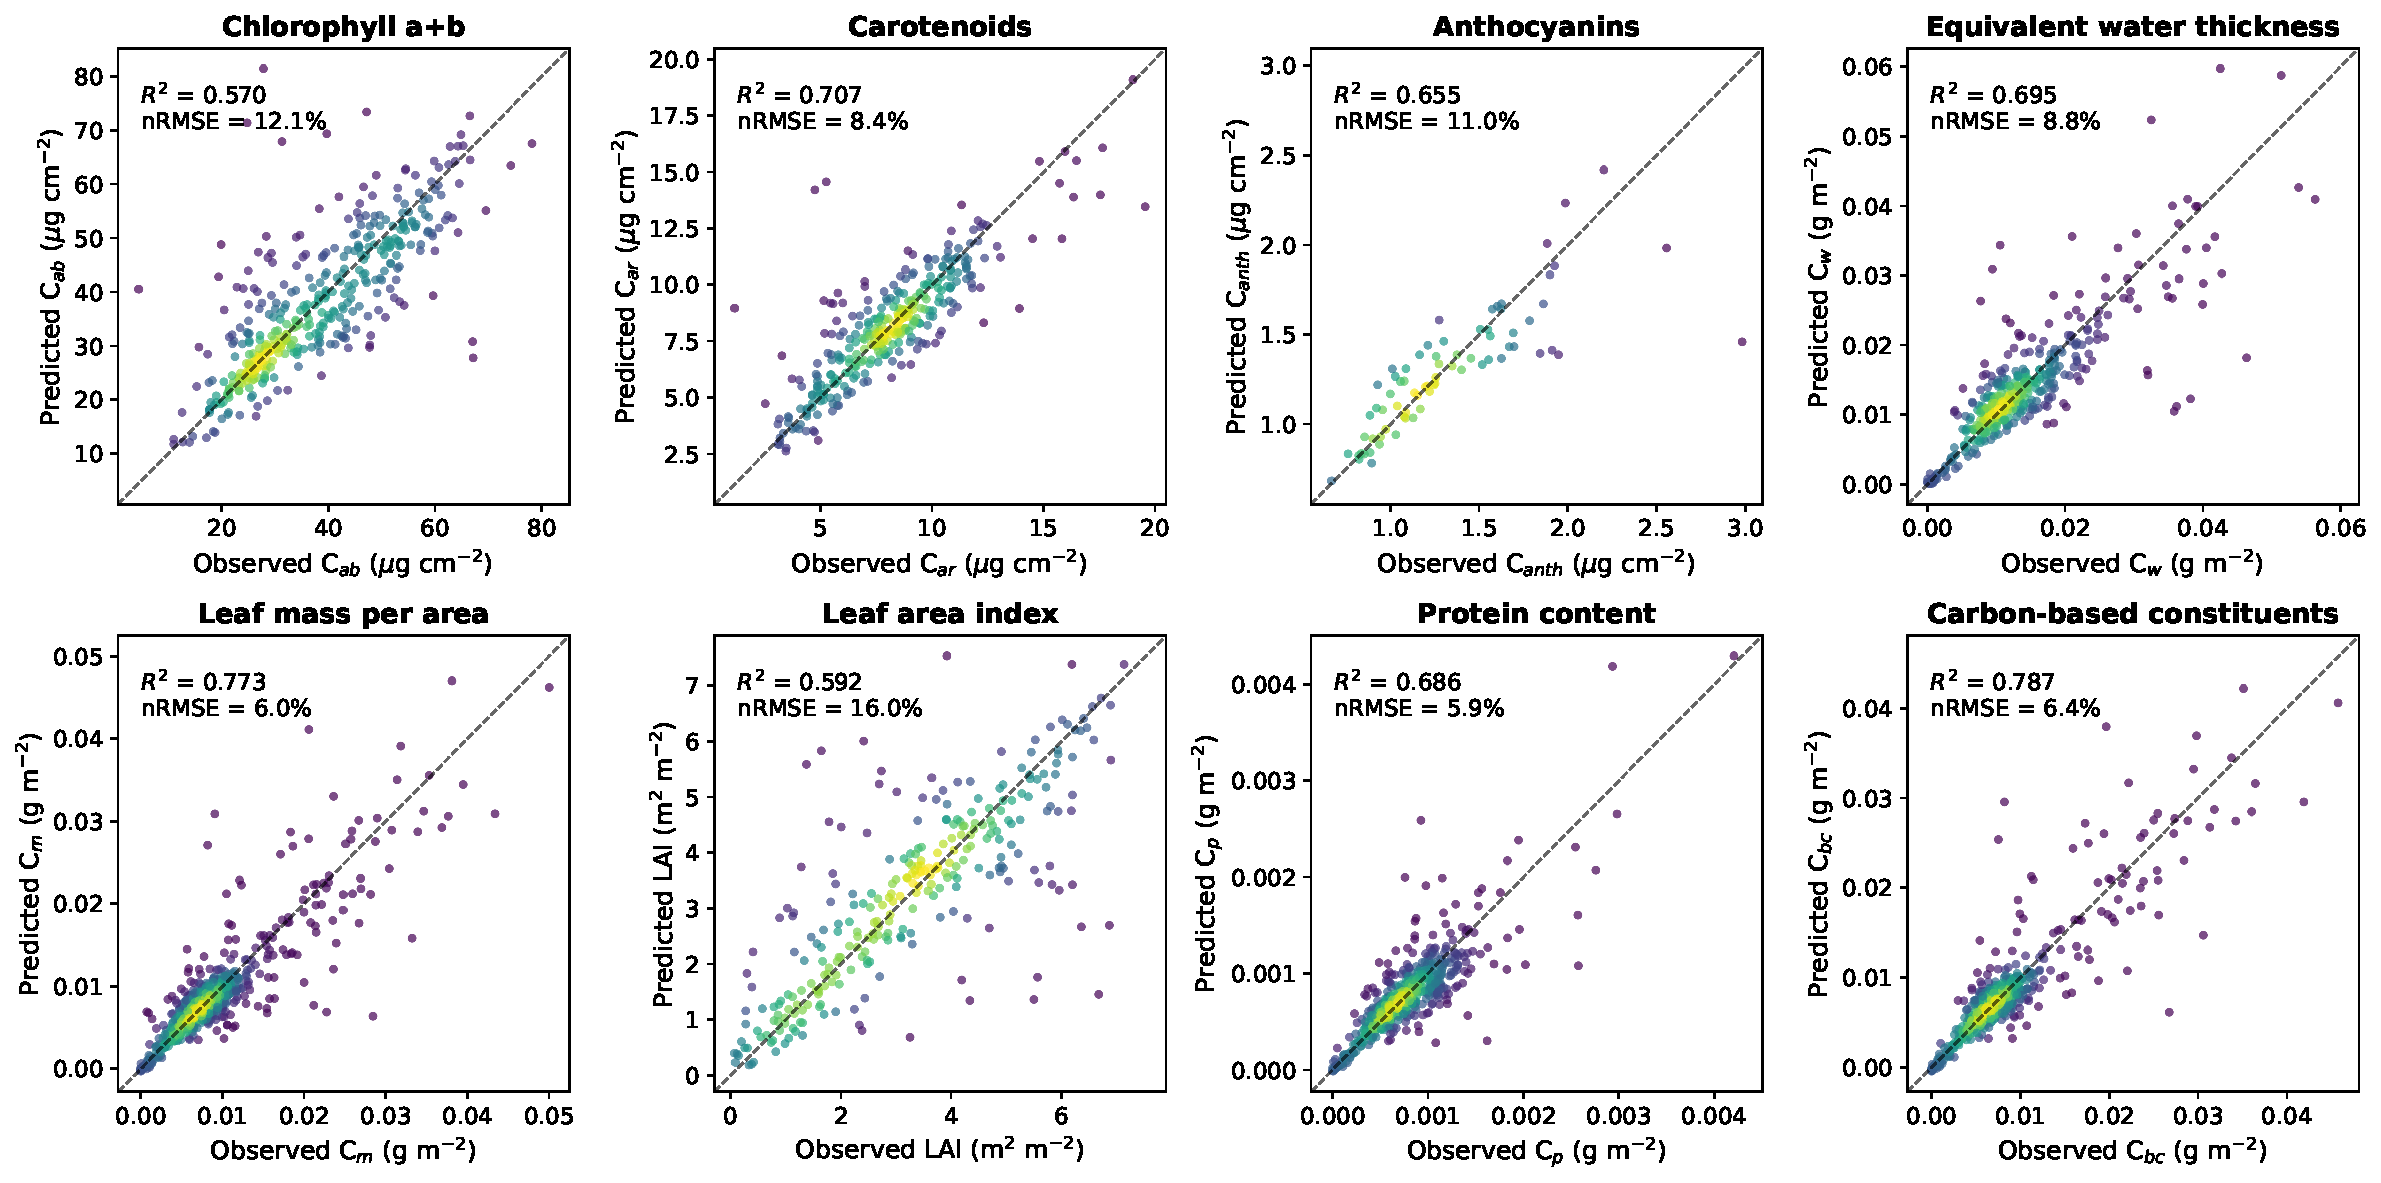
\includegraphics[width=\textwidth]{figures/scatterplot_best_model.pdf}
    \caption{Observed versus predicted trait values for the supervised 2D model (Reshape + EfficientNet-B0) on the GreenHyperSpectra test set ($n = 1{,}127$). Points are coloured by kernel density estimation. The dashed line represents the 1:1 relationship. $R^2$ and RMSE are reported for each trait. Not all test samples have measurements for every trait.}
    \label{fig:scatterplot}
\end{figure}

\subsection{Case Study 2: Self-Supervised Pretraining}
\label{sec:results_pretraining}

Table~\ref{tab:pretraining} compares the performance of supervised and self-supervised approaches across 1D and 2D representations. Among 1D methods reported by \citet{cherif2025greenhyperspectra}, the masked autoencoder with fine-tuning (MAE-1D FT) achieved the best performance ($R^2 = 0.645$), outperforming the supervised baseline by +0.058 and confirming the value of self-supervised pretraining on the 139,295 unlabeled spectra available in GreenHyperSpectra. The semi-supervised SR-GAN and physics-informed RTM-AE achieved only marginal improvements over the supervised baseline (+0.005 each).

Our 2D supervised approach (Reshape + EfficientNet-B0, $R^2 = 0.684 \pm 0.001$) surpassed all 1D methods, including the best self-supervised MAE-1D FT, by a margin of +0.039. This result demonstrates that the representational advantage conferred by 2D spectral images exceeds the benefit of self-supervised pretraining within the 1D framework. The MAE-2D with fine-tuning ($R^2 = 0.667 \pm 0.006$) also outperformed the 1D MAE-FT by +0.022, confirming that the 2D advantage extends to the self-supervised setting. However, the MAE-2D did not surpass the supervised 2D baseline, suggesting that with the current labeled dataset size ($n = 4{,}508$), the pretrained representations do not provide sufficient additional information beyond what direct supervised learning captures.

\begin{table}[htbp]
\centering
\caption{Comparison of pretraining strategies. All 2D methods use the Reshape transformation. Cherif baselines are from \citet{cherif2025greenhyperspectra}. Mean $R^2$ and standard deviation across three seeds are reported where available.}
\label{tab:pretraining}
\begin{tabular}{llcc}
\toprule
Method & Type & Mean $R^2$ $\pm$ std & $\Delta$ vs.\ Supervised 1D \\
\midrule
\multicolumn{4}{l}{\textit{Cherif et al.\ (2025) --- 1D baselines}} \\
Supervised EfficientNet-1D   & Supervised       & 0.587 $\pm$ 0.004 & -- \\
SR-GAN                        & Semi-supervised  & 0.592 $\pm$ 0.003 & +0.005 \\
RTM-AE                        & Physics-informed & 0.592 $\pm$ 0.004 & +0.005 \\
MAE-1D Linear Probing         & Self-supervised  & 0.604 $\pm$ 0.005 & +0.017 \\
MAE-1D Fine-Tuning            & Self-supervised  & 0.645 $\pm$ 0.003 & +0.058 \\
\midrule
\multicolumn{4}{l}{\textit{Ours --- 2D methods}} \\
\textbf{Supervised 2D (Reshape)} & Supervised    & \textbf{0.684 $\pm$ 0.001} & \textbf{+0.097} \\
MAE-2D Fine-Tuning            & Self-supervised  & 0.667 $\pm$ 0.006 & +0.080 \\
\bottomrule
\end{tabular}
\end{table}


The observation that supervised 2D training outperforms MAE-2D fine-tuning warrants further consideration. The MAE-2D encoder (ViT-Tiny, 2.8M parameters) is architecturally distinct from the supervised model (EfficientNet-B0, 4.0M parameters), and the gap may partly reflect the superior inductive biases of convolutional architectures for this image size and dataset scale. Additionally, the MAE pretraining converged rapidly (within approximately 10 epochs), with reconstruction loss approaching zero, suggesting that the 224$\times$224 Reshape images may not present sufficient reconstruction complexity to learn richly discriminative representations. Future work could explore larger encoder architectures, alternative masking strategies, or multi-scale patch sizes to improve the quality of pretrained features.

\section{Discussion}
\label{sec:discussion}

\subsection{Why reshaping spectra into images improves trait retrieval}
\label{sec:disc_reshape}

% --- Opening: headline finding in context ---
 - This study demonstrates that a simple reshape of 1D
   hyperspectral reflectance into a 2D image significantly
   improves multi-trait retrieval ($R^2 = 0.684$ vs 0.587
   for supervised 1D-CNN)
 - Consistent across all eight traits --- no trait is
   degraded by the 2D representation
 - Reshape outperformed five alternative transformations,
   confirming prior findings that direct reshaping is
   competitive or superior to engineered encodings
   \citep{hennessy2022reshaping, deev2024spectrum,
   sharma2019deepinsight}, and extending this to
   multi-trait regression with heterogeneous field data

% --- Mechanism: multi-scale receptive field ---
 - The $42 \times 42$ reshape creates a topology where a
   single $3 \times 3$ kernel spans $\sim$84\,nm of
   spectral range (vertical stride of 42\,nm), versus
   $\sim$3\,nm for an equivalent 1D kernel
 - After a few pooling stages in EfficientNet-B0, the
   effective receptive field covers hundreds of nm ---
   enough to simultaneously capture pigment absorption
   at 680\,nm, the red-edge at 750\,nm, and SWIR
   structural features
 - In a 1D-CNN, achieving the same spectral reach
   requires very deep networks or large kernels ($k > 80$),
   increasing overfitting risk with limited labeled data
   ($n = 4{,}508$) \citep{cherif2023spectra}
 - The reshaped image also encodes trait-specific
   ``spectral textures'' --- visually distinct spatial
   patterns arising from different biochemical
   compositions (Figure~\ref{fig:transforms_example}) ---
   that 2D convolutions are specifically designed to
   detect

% --- Per-trait evidence supports the mechanism ---
 - The per-trait improvement gradient directly supports
   the cross-band correlation mechanism
 - Largest gains for traits with broad, distributed
   absorption features:
   C$_\text{bc}$ ($\Delta R^2 = +0.245$, carbon-based
   constituents absorbing across 1700--2300\,nm),
   Anth ($\Delta = +0.174$, interacting with chlorophyll
   features $\sim$80--180\,nm apart),
   and C$_\text{m}$ ($\Delta = +0.122$, dry matter
   spanning multiple SWIR windows)
   \citep{curran1989imaging, feret2021prospectpro}
 - Moderate gains for pigments (C$_\text{ab}$
   $\Delta = +0.080$, C$_\text{ar}$ $\Delta = +0.070$):
   narrower visible-range features already partially
   captured by 1D convolutions, though 2D adds
   correlations with red-edge and NIR regions
   \citep{homolova2013review}
 - Near-zero gain for C$_\text{p}$ ($\Delta = +0.008$):
   protein has a narrow absorption at $\sim$2100\,nm
   \citep{feret2021prospectpro} --- cross-band
   correlations add minimal information for spectrally
   confined signals
 - This gradient (broad features $\rightarrow$ largest
   gains; narrow features $\rightarrow$ smallest gains)
   is consistent with the hypothesis that the 2D
   advantage arises from multi-scale cross-band
   integration

% --- Why complex transforms underperform ---
 - CWT ($R^2 = 0.641$) and Spectrogram ($R^2 = 0.636$)
   formed a second tier --- both preserve some spectral
   locality through windowed decomposition
   \citep{addison2017wavelet, shuai2025multichannel},
   but placing wavelength on one axis and scale/frequency
   on the other breaks the wavelength-to-wavelength
   adjacency that Reshape preserves
 - These transforms have proven effective for
   classification tasks where scale-specific
   discriminative features matter
   \citep{ong2025sugarcane, zhuang2023cwt,
   shuai2025multichannel, zhang2025gaf}, but for
   continuous regression the direct wavelength topology
   appears more informative
 - GAF ($R^2 = 0.609$) maps spectral values to angular
   space, grouping bands by reflectance magnitude rather
   than wavelength position, thus losing the physical
   ordering that connects absorption features to
   biochemistry \citep{wang2015gaf, ganesan2021gaf};
   GAF and MTF were designed for time-series
   classification where phase dynamics carry
   discriminative information --- a fundamentally
   different task
 - 2D-COS ($R^2 = 0.555$, std $= 0.077$) showed the
   highest seed variability; our single-sample adaptation
   via windowed segmentation \citep{noda2004twodimensional}
   is an ad-hoc perturbation that may introduce noise
   rather than meaningful correlation structure
 - MTF ($R^2 = 0.419$) was the only transform worse than
   the 1D baseline --- quantile-based discretisation
   destroys continuous spectral information critical for
   regression \citep{wang2015gaf}
 - Overall: transforms preserving natural wavelength
   ordering and continuous values outperform those
   remapping spectral information into abstract
   mathematical spaces


\subsection{\jl{What the model learns from the 2D representation}}
\label{sec:disc_importance}

% --- 2D importance makes the receptive-field mechanism empirical ---
\jl{ - The variable importance analysis gives empirical
   support to the receptive-field mechanism proposed in
   Section~\ref{sec:disc_reshape}. Grad-CAM relevance
   forms compact 2D clusters. Once unfolded to wavelength,
   six of the eight traits concentrate importance in known
   absorption regions above chance
   (Figure~\ref{fig:importance}).}

\jl{ - The unfolded maps expose how the model reads the
   image. Horizontal neighbours are adjacent bands.
   Vertical neighbours are bands 42 positions apart. A
   single 2D kernel reads both at once. The model can
   co-weight a visible feature and its shortwave-infrared
   overtone about 42 bands away inside one receptive
   field. A 1D kernel of the same size cannot.}

\jl{ - Integrated Gradients and Grad-CAM agree. IG works at
   the fine, signed, band level. Grad-CAM works at the
   coarse, region level. Their agreement raises confidence
   that the importance reflects learned spectral structure
   rather than an artifact of one method.}

% --- Relation to known absorption regions and why they differ ---
\jl{ - Six traits concentrate importance in physically
   grounded regions. Anthocyanins, leaf mass per area,
   carbon-based constituents, chlorophyll, and protein all
   stay above chance. Their peaks fall on the red-edge
   (C\textsubscript{ab} at 703\,nm) and on shortwave-infrared
   cellulose, lignin, and protein features (near 2144\,nm).
   These match constituent absorption reported at the leaf
   level \citep{serbin2020scaling, angel2022remote,
   curran1989imaging, feret2021prospectpro}.}

\jl{ - These windows come from constituent absorption
   physics, not from the model. Pigment electronic
   transitions in the visible, and water, protein,
   cellulose, and lignin vibrational overtones in the
   shortwave infrared, occupy stable wavelength ranges
   across studies \citep{curran1989foliar, fourty1996leaf,
   feret2021prospectpro}. They are independent of the
   retrieval method. Band importance derived from the model
   itself shifts with the algorithm, the regularisation,
   and the training data. We compared against the physical
   regions to keep the reference independent of our model.}

\jl{ - Carotenoids ($0.82\times$) and equivalent water
   thickness ($0.81\times$) fall below chance. The model
   predicts both well, so the mismatch reflects where the
   model looks rather than how well it performs. Several
   non-exclusive reasons explain the difference from the
   literature.}

\jl{ - Scale differs. The reference regions come from leaf
   or constituent spectra. GreenHyperSpectra holds canopy
   reflectance. Canopy structure, leaf area index, soil
   background, and multiple scattering broaden, shift, and
   saturate absorption features. The predictive bands need
   not match the leaf-level maxima \citep{homolova2013review}.}

\jl{ - Traits covary. The multi-trait model can predict a
   weakly featured trait through a correlated strong one.
   Carotenoids share variance with chlorophyll. The model
   leans on the chlorophyll red-edge at 703\,nm rather than
   the weak carotenoid feature at 440--520\,nm. A good
   R\textsuperscript{2} of 0.707 with low enrichment reflects
   this shortcut.}

\jl{ - Preprocessing removed water bands. The strongest
   water features near 1450 and 1940\,nm fall partly inside
   the removed gaps (1351--1430 and 1801--2050\,nm). The
   model uses the surviving edge at 1431\,nm. The low water
   enrichment is partly a preprocessing artifact, not
   biology.}

\jl{ - The metric depends on our window choice. We set the
   absorption windows from the literature. Narrow windows
   penalise the legitimate use of adjacent bands and lower
   the enrichment for traits with broad or shifted
   features.}


\subsection{Self-supervised pretraining in the 2D framework}
\label{sec:disc_pretraining}

% --- Key comparison ---
 - The 2D supervised baseline ($R^2 = 0.684$) surpassed
   all 1D methods, including the best self-supervised
   MAE-1D FT ($R^2 = 0.645$) of
   \citet{cherif2025greenhyperspectra}
 - The representational advantage of 2D images alone
   (+0.039 over MAE-1D FT) exceeds the benefit of
   pretraining on 139K unlabeled spectra within the 1D
   framework (+0.058 over supervised 1D)
 - The 2D representation is therefore the dominant factor,
   not the learning strategy

% --- MAE-2D results ---
 - MAE-2D FT ($R^2 = 0.667 \pm 0.006$) outperformed
   MAE-1D FT by +0.022, confirming the 2D advantage
   extends to self-supervised learning
 - However, MAE-2D FT did not surpass supervised 2D
   ($-0.017$), contrasting with natural image domains
   where MAE pretraining typically helps \citep{he2022mae}
 - Linear probing ($R^2 = 0.646 \pm 0.020$, only 38.6K
   trainable parameters) exceeded all 1D baselines
   including MAE-1D FT --- capturing 97\% of fine-tuned
   performance and indicating the frozen encoder already
   encodes most trait-relevant spectral information

% --- Why supervised 2D > MAE-2D FT ---
 - Three non-mutually exclusive hypotheses:
   (1) Architecture mismatch --- EfficientNet-B0's spatial
   inductive biases (local connectivity, translation
   equivariance) outperform ViT's learned attention with
   only $n = 4{,}508$ labeled samples
   \citep{dosovitskiy2021vit};
   (2) Easy reconstruction --- reshaped spectral images
   have smooth, continuous structure unlike natural images,
   so the MAE task converges rapidly ($\sim$10 epochs,
   val\_loss $\sim$0.0001) without learning deep
   trait-discriminative features;
   (3) Sufficient labeled data --- 4,508 samples spanning
   diverse ecosystems may already capture most learnable
   spectral--trait relationships
 - Practical implication: researchers can achieve
   state-of-the-art performance with reshape + standard
   CNN, without the computational cost of pretraining on
   large unlabeled corpora
 - The MAE-2D result remains valuable for data-scarce
   settings where few labeled samples are available


\subsection{Implications for trait-based ecology and remote sensing}
\label{sec:disc_implications}

% --- Carbon cycle and ecosystem functioning ---
 - The largest improvement was for C$_\text{bc}$
   ($\Delta R^2 = +0.245$), directly linked to carbon
   stocks, litter decomposition, and nutrient cycling
   \citep{kattge2020try}
 - Improved C$_\text{bc}$ and C$_\text{m}$ retrieval
   supports non-destructive estimation of leaf dry
   matter investment --- a key axis of the leaf economics
   spectrum \citep{wright2004les} --- enabling more
   reliable mapping of ecosystem carbon pools and
   decomposition dynamics for Earth system models
   \citep{homolova2013review}

% --- Functional diversity monitoring ---
 - Multi-trait retrieval from a single model preserves
   inter-trait covariance structure, essential for
   functional diversity metrics (FDis, FRic, FEve, Rao's
   Q) \citep{villeger2008fd, laliberte2010fdis}
 - Trait-by-trait retrieval with independent models may
   distort correlations and bias diversity estimates
 - Simultaneous improvement across all eight traits means
   functional trait spaces from 2D predictions will be
   more accurate and internally consistent than 1D
   baselines --- relevant for biodiversity monitoring
   programmes relying on spectral trait mapping
   \citep{schweiger2018plant, binh2025mangrove, weiss2020remote}

% --- Operational simplicity ---
 - Reshape requires no domain-specific tuning (no wavelet
   scales, STFT windows, quantile bins, or perturbation
   parameters) and is implementable in $\sim$6 lines of
   code
 - Robustness across seeds (std $= 0.001$) ensures
   reproducible results without hyperparameter sensitivity
 - This lowers the barrier for ecologists and remote
   sensing practitioners who need state-of-the-art
   predictions without signal processing expertise

% --- Scaling to hyperspectral missions ---
 - Upcoming and recently launched missions --- EnMAP
   \citep{guanter2015enmap}, PRISMA
   \citep{verrelst2021prisma}, SBG/EMIT
   \citep{cawse2021sbg, green2020emit} --- will produce continental-
   to global-scale hyperspectral archives with contiguous
   spectra across 400--2500\,nm
 - A simple, robust method validated across 50
   heterogeneous datasets is well suited for operational
   deployment on these data streams

% --- Data-efficient learning for undersampled biomes ---
 - The MAE-2D linear probe ($R^2 = 0.646$, 38.6K params)
   opens a pathway for trait prediction in data-scarce
   biomes (tropical forests, tundra, peatlands) that are
   underrepresented in existing trait databases
   \citep{kattge2020try, zhang2025ppadanet}
 - A frozen pretrained encoder requiring only a
   lightweight linear head could enable trait mapping
   with minimal local calibration data, aligning with the
   broader trend toward foundation models for remote
   sensing \citep{binfaruk2025terramae}


\subsection{Limitations and future directions}
\label{sec:disc_limitations}

% --- Methodological limitations ---
 - All transform comparisons used a single backbone
   (EfficientNet-B0); performance rankings could differ
   with other architectures, though
   \citet{cherif2023spectra} showed it to be optimal for
   this data scale
 - Fixed image size ($224 \times 224$): the reshape
   topology depends on resolution, and other sizes may
   favour different transforms --- a systematic study is
   warranted
 - Single-sample 2D-COS via windowed segmentation is an
   ad-hoc approximation of \citet{noda2004twodimensional}'s
   multi-sample formulation --- its poor performance may
   partly reflect this limitation
 - All experiments used GreenHyperSpectra; validation on
   independent datasets with different spectral
   resolutions, wavelength ranges, and ecosystem types is
   needed
 - The moderate labeled set ($n = 4{,}508$) may limit the
   benefit of self-supervised pretraining; with larger
   datasets, the gap between supervised and MAE-2D could
   narrow
 - This study used point-level spectra without spatial
   context --- airborne/satellite imagery introduces mixed
   pixels and atmospheric effects not addressed here

\jl{ - The Reshape geometry is arbitrary, which limits the
   importance maps. The model zero-pads the spectrum and
   resizes it bilinearly from $42 \times 42$ to
   $224 \times 224$, smearing each band over about five
   pixels. The vertical 42-band adjacency comes from the
   $\text{side} = 42$ fold, not from physics, so part of
   the cross-row structure reflects the layout. The
   unfolded importance has limited spectral resolution and
   the apparent peaks can shift by a few bands. Row-wrap
   boundaries place spectrally adjacent bands far apart in
   the image. We therefore read the importance maps as
   approximate.}

% --- Future directions ---
 - Investigate the effect of image size and reshape
   topology on retrieval --- different row widths create
   different cross-band neighborhoods that may favour
   different traits
 - Explore harder MAE pretraining: higher mask ratios,
   structured masking of spectral regions, and CWT
   scalograms as inputs (richer spatial structure than
   reshape)
 - Pretrain larger 2D encoders on massive spectral
   archives for general-purpose spectral feature
   extraction (foundation models)
 - Combine reshaped spectral images with spatial context
   from imaging spectrometers or LiDAR-derived canopy
   structure (multi-modal fusion)


\input{Chapters/Conclusion}


% Bibliography settings
\bibliographystyle{elsarticle-harv}
\bibliography{References}

\end{document}